\begin{frame}[t,fragile]{単純サンプリング}
  \begin{itemize}
    \setlength{\itemsep}{1em}
  \item $[0,c]$ と $[0,2]$ の一様分布から二次元上の点 $(x,y)$ を $M$ 組生成
  \item $f(x)$ の下に入った数 $N$ をカウント
    \[
    \pi \simeq 2c \times \frac{N}{M}
    \]
    \begin{tabular}{|c|c|c|}
      \hline
      $M$ & 平均値 & 誤差 \\
      \hline
      100 & 4.8 & 1.3 \\
      10000 & 3.12 & 0.11 \\
      1000000 & 3.154 & 0.011 \\
      \hline
    \end{tabular}
  \end{itemize}
  \vspace*{-7em}
  \hspace*{17em}
  \resizebox{!}{.45\textheight}{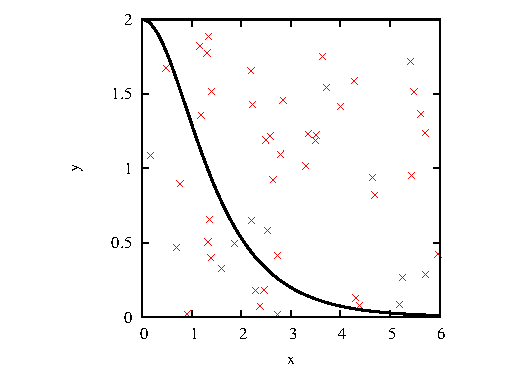
\includegraphics{image/coth-1.pdf}}
\end{frame}
